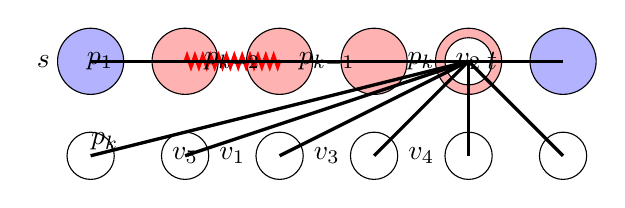
\begin{tikzpicture}[scale=0.6]
\filldraw[fill=blue!30!white,draw=black] (-8,-1) circle (0.7);
\filldraw[fill=red!30!white,draw=black] (-6,-1) circle (0.7);
\filldraw[fill=red!30!white,draw=black] (-4,-1) circle (0.7);
\filldraw[fill=red!30!white,draw=black] (-2,-1) circle (0.7);
\filldraw[fill=red!30!white,draw=black] (-0,-1) circle (0.7);
\filldraw[fill=white,draw=black] (0,-3) circle (0.5);
\filldraw[fill=white,draw=black] (-2,-3) circle (0.5);
\filldraw[fill=white,draw=black] (-4,-3) circle (0.5);
\filldraw[fill=white,draw=black] (0,-1) circle (0.5);
\filldraw[fill=white,draw=black] (-8,-3) circle (0.5);
\filldraw[fill=white,draw=black] (2,-3) circle (0.5);
\filldraw[fill=blue!30!white,draw=black] (2,-1) circle (0.7);
\filldraw[fill=white,draw=black] (-6,-3) circle (0.5);

\draw[very thick,red,decoration={zigzag,segment length=1mm, amplitude=0.7mm},decorate] (-6,-1) -- (-4,-1);
\draw[very thick,red] (-8,-1) -- (-6,-1);
\draw[very thick] (-4,-1) -- (-2,-1);
\draw[very thick] (-2,-1) -- (-0,-1);
\draw[very thick] (-0,-1) -- (-8,-3);
\draw[very thick] (-0,-1) -- (-2,-3);
\draw[very thick] (-0,-1) -- (-4,-3);
\draw[very thick] (-0,-1) -- (0,-3);
\draw[very thick] (-0,-1) -- (2,-3);
\draw[very thick] (-0,-1) -- (-6,-3);
\draw[very thick] (-0,-1) -- (-8,-1);
\draw[very thick] (-0,-1) -- (2,-1);

\draw (-9,-1) node {$s$};
\draw (-7.8,-1) node {$p_1$};
\draw (-5,-1) node {$p_{k-2}$};
\draw (-3,-1) node {$p_{k-1}$};
\draw (-1,-1) node {$p_k$};
\draw (0.5,-1) node {$t$};
\draw (-7.7,-2.7) node {$p_k$};
\draw (-5,-3) node {$v_1$};
\draw (-3,-3) node {$v_3$};
\draw (-1,-3) node {$v_4$};
\draw (0,-1) node {$v_2$};
\draw (-6,-3) node {$v_5$};

\end{tikzpicture}